\documentclass[UTF8,a4paper,12pt]{ctexart}

\usepackage[margin=1in]{geometry}
\usepackage{graphicx}
\usepackage{amsmath}
\usepackage{amssymb}
\usepackage{booktabs}
\usepackage{longtable}
\usepackage{array}
\usepackage{tabularx}
\usepackage{float}
\usepackage{url}
\usepackage{hyperref}
\usepackage{setspace}

\hypersetup{
    colorlinks=true,
    linkcolor=black,
    citecolor=black,
    urlcolor=blue
}

\setlength{\parindent}{2em}
\setlength{\parskip}{0.3em}
\setstretch{1.25}
\graphicspath{{Figures/}{../Results/0020_results/}{../Results/0020_results/Online/}{../Results/0020_results/Offline/}}

\title{ME5400 课程项目技术报告\\基于 FAST-LIO、PointPillars 与 MCTrack 的动态场景双向协同定位跟踪系统}
\author{ME5400 Project}
\date{\today}

\begin{document}
\maketitle

\begin{abstract}
本报告面向 ME5400 高级机器人与自主系统课程项目，系统总结一个基于 LiDAR 与 IMU 的动态场景 SLAM--MOT 融合管线。项目围绕一个很直接但又长期存在的工程问题展开：在自动驾驶场景中，道路上的车辆既会破坏激光雷达建图与定位，又是最重要的动态目标；如果只把它们当成离群点过滤掉，定位系统虽然更稳定，但跟踪与建图之间没有形成真正的信息闭环，动态目标也没有被充分利用。为此，本项目构建了一套覆盖前端感知、中端双向融合、后端联合优化和离线工程调度的完整 ROS 管线：以前端 PointPillars 完成三维目标检测，以 FAST-LIO 提供高频激光惯性里程计，以 MCTrack 完成多目标跟踪与速度估计，再将跟踪结果反向馈入 FAST-LIO 做动态点自适应降权，并进一步送入 ego-only 滑窗联合后端对自车位姿进行再优化。系统的核心思想并不是简单地把多个模块串联起来，而是让定位结果显式帮助目标跟踪，让跟踪结果再反过来帮助定位与建图，从而形成一个面向动态场景的闭环协同架构。基于仓库当前归档实验结果，系统在 KITTI Tracking 多个序列上取得了可观收益，其中序列 0020 的 ATE RMSE 从 29.1782\,m 降至 11.5856\,m，改善 60.29\%；KITTI 相对平移误差从 6.0245\% 降至 2.9930\%，改善 50.32\%。报告还结合项目内的 \texttt{slammot\_comparison.md} 对近期 SLAMMOT 方向的代表性工作进行了定位分析，说明本项目与紧耦合因子图方法之间的差异、当前系统的工程价值，以及后续朝着“将动态物体从干扰源转化为移动路标”的 object-centric LiDAR-inertial 联合优化方向演进的潜力。
\end{abstract}

\noindent\textbf{关键词：} FAST-LIO；PointPillars；MCTrack；动态场景 SLAM；多目标跟踪；LiDAR-inertial odometry；ROS

\section{引言}
动态场景定位与感知的矛盾，是自动驾驶与移动机器人系统中最典型、也最难彻底解决的一类问题。经典的激光 SLAM 或 LIO 系统通常默认环境中绝大部分结构是静态的，因此它们在前端配准、地图维护、误差状态滤波和后端优化时都倾向于把“能够长期复用的静态几何结构”视为主要信息来源。然而真实道路并非如此。城市道路与高速路上持续出现的车辆、行人、自行车和大型动态目标，会在点云中产生大量时变结构。当这些动态点被错误地当成静态结构写入地图，系统就会出现常见的动态鬼影、局部配准偏移、累计漂移加剧、回环前地图污染等问题。另一方面，如果系统采取非常保守的策略，将所有可能动态的区域一概剔除，虽然能缓解建图污染，但可用几何约束也会被同步削弱，尤其在道路边界稀疏、高速行驶或视角急剧变化时，定位稳定性并不一定更好。

与此同时，多目标跟踪系统也面临与之对偶的困难。以 3D MOT 为代表的目标跟踪任务，在本质上依赖于跨帧检测框之间的一致关联。为了完成可靠的数据关联，跟踪器需要知道“同一个目标在下一帧大致会出现在什么位置”。如果自车本身正在转弯、加减速或者发生姿态扰动，而跟踪器没有获得足够精确且高频的自车运动补偿，那么检测框的跨帧几何关系就会被自车运动扰乱，导致轨迹中断、ID Switch、速度估计不稳定甚至错误删轨。因此，在自动驾驶系统中，定位模块与跟踪模块事实上互相需要：定位越准确，目标跟踪越稳定；跟踪越稳定，系统越有可能识别出哪些点来自运动目标，从而反向提升定位与建图。

本项目正是沿着这一思路展开。与许多“把 SLAM 和 MOT 放在同一论文中但仍各做各的”的工程组合不同，ME5400 项目尝试构造一个真正具有双向信息流的闭环管线。项目基于仓库现有实现，形成了从数据输入到评估输出的完整 ROS 生态：原始 KITTI rosbag 提供 LiDAR 与 IMU；PointPillars 检测器输出三维车辆框；FAST-LIO 提供优化位姿与 IMU 预测位姿；MCTrack 接收检测与位姿后完成在线多目标跟踪；跟踪结果既反馈给 FAST-LIO 做动态目标降权，也进一步送入联合后端，作为修正自车轨迹的软约束。换言之，这个系统不是单纯地“在 FAST-LIO 后面加一个跟踪器”，也不是“在检测之后加一个可视化节点”，而是在现有成熟模块基础上构建了一个面向动态场景的协同框架。

如果从研究背景的角度理解这个项目，其意义还不仅仅在于提升若干个具体序列上的误差指标。根据项目中的 \texttt{slammot\_comparison.md} 对近期代表性 SLAMMOT 类工作的总结，不少工作已经开始讨论动态环境下的联合建图与目标跟踪，例如 Conf SLAMMOT、LIMOT、IMM-SLAMMOT、Online Dynamic SLAM、DL-SLOT 等。这些工作在传感器配置、优化框架、数据关联与运动模型等方面各有侧重，但总体上具有三个共性。第一，它们普遍意识到 SLAM 与 MOT 之间不应完全解耦，至少在后端或者滑窗层面应当共享一部分变量或约束。第二，它们几乎都承认动态物体不能简单视作噪声，而应当被建模、过滤、跟踪或联合优化。第三，它们中的多数仍然没有把“动态物体几何结构本身”真正转化为能帮助自车定位的可利用信息，更多还是在做动态物体过滤、目标状态联合估计或隐式数据关联。也就是说，“动态目标从干扰源转变为移动路标”这一更激进也更有潜力的方向，仍然存在明显空白。

ME5400 当前实现并未完全走到这一步，但它已经在工程上向这个方向迈出了关键的一步。它首先建立了完整的前端检测、里程计、跟踪与后端优化通信接口；其次在 FAST-LIO 内部完成了动态目标感知下的点云降权，而不是仅靠独立预处理过滤；再次在 ego-only 联合后端中引入了来自跟踪目标的观测一致性约束，使动态目标不只“被避开”，而是开始“被用来帮助修正自车位姿”；最后，项目以统一脚本、离线 feeder、评估图表与多序列结果归档的方式，形成了课程项目中少见的完整可运行验证闭环。这些特征决定了它既是一个工程系统，也是一个具有研究延展空间的原型平台。

需要特别说明的是，仓库根目录的 README 中曾给出过一组序列 0020 的示例结果，例如 RMSE 从 21.44\,m 降至 5.46\,m 的数据；而当前 \texttt{Results/} 中还保存了另一组更完整的联合后端实验结果。由于这些数字来自不同时间的归档运行，本报告在实验章节中统一采用仓库当前可核对的结果文件，尤其是 \texttt{metrics\_joint\_backend.txt} 与 \texttt{metrics\_kitti\_tr\_rot\_ac.txt} 中的指标，以保证报告内容与可复现实验输出一致。

基于上述背景，本报告的目标有三点。第一，完整梳理项目的系统架构与数据流，不仅解释“用了哪些模块”，更解释这些模块为什么这样连接。第二，系统阐述项目中已经落地的方法细节，包括 PointPillars 检测节点、FAST-LIO 动态降权、MCTrack 在线时序对齐与联合后端优化。第三，结合真实归档实验，分析当前系统在哪些序列上有效、为什么有效、在哪些场景下仍会失败，以及未来应如何从工程型松耦合系统继续走向更强的 object-centric 紧耦合联合优化框架。

\section{相关工作与项目定位}
如果把本项目放到更大的 SLAMMOT 研究脉络中观察，可以发现它与当前主流工作既有相似之处，也有非常明确的定位差异。根据项目内部整理的 \texttt{slammot\_comparison.md}，近期相关工作大体可以分为两类。一类是围绕联合因子图或滑窗优化构建的紧耦合系统，例如 LIMOT、Conf SLAMMOT、DL-SLOT 等。这类方法通常把自车位姿、目标位姿、观测关联和运动模型放入统一优化框架中，理论上更完整，也更容易从概率图优化角度建立统一解释。另一类则更强调特定传感器模态下的动态环境处理，例如视觉侧的 IMM-SLAMMOT、Online Dynamic SLAM、VDO-SLAM、DynaSLAM II 等，它们往往在实例分割、动态物体建模、增量优化或多运动模型方面做得更细。

这些工作的共同趋势说明两个事实。其一，动态场景 SLAM 不再满足于“先分割动态点，再套静态 SLAM”这样简单的串联范式。其二，多目标跟踪也不再只是独立于定位系统的感知后处理模块，而是越来越多地与位姿估计共享信息。然而如果进一步比较，就会发现仍存在几个关键空白。

首先，真正建立在高质量 LiDAR-inertial 前端之上的联合系统仍不多。视觉动态 SLAM 相关文献非常丰富，但视觉系统在光照、纹理缺失和尺度漂移方面具有天然脆弱性，而自动驾驶真实落地更看重 LiDAR 与 IMU 的鲁棒性。FAST-LIO 作为高性能 LiDAR-inertial 里程计前端，本身具备极强的实时性和工程成熟度。如果能够在 FAST-LIO 基础上叠加动态目标利用机制，就比“从头自研一个定位前端”更现实，也更容易复用已有工程资产。

其次，大多数系统虽然声称同时处理了 SLAM 与 MOT，但动态物体在系统中往往仍然被更多地视作“需要被过滤或跟踪的对象”，而不是“能够回过头来帮助定位的几何参照”。例如，有些方法通过检测或分割把动态点从地图优化中移除；有些方法在联合图中显式优化目标轨迹，但重点仍然是提高目标跟踪性能；还有些方法利用目标运动模型约束短时一致性，却没有真正把车辆表面或刚体运动的稳定结构用作自车定位的额外信息。项目笔记中已经明确指出，这种“把动态物体从毒瘤变成路标”的思路在视觉领域有零星启发，但在 LiDAR-inertial 框架下尚缺少成熟实现。

再次，很多论文级系统在理论层面紧耦合，但工程落地成本高、ROS 集成弱、调试链路复杂。相反，ME5400 当前版本的价值恰恰在于它是一个模块化、可运行、可视化、可批量验证的完整工程框架。它采用松耦合设计，通过 topic 通信把检测、跟踪、前端里程计和联合后端串起来。这种设计不如统一因子图“优雅”，但对于课程项目和快速验证而言具有很强的可维护性。PointPillars、MCTrack、FAST-LIO 都是相对成熟的现成模块，项目所做的工作并不是重复发明它们，而是建立它们之间的协同接口、补足时序对齐与消息转换，并在关键位置加入动态场景下的新机制。

因此，本项目的定位应当理解为：它不是一个“最终版”的紧耦合 SLAMMOT 研究系统，而是一个已经完成闭环协同验证的工程型原型平台。与 LIMOT、Conf SLAMMOT 之类方法相比，它当前仍然更偏松耦合；与 VDO-SLAM、DynaSLAM II 等视觉动态 SLAM 相比，它使用 LiDAR + IMU，更偏向几何与运动鲁棒性；与纯检测或纯跟踪系统相比，它又显式把目标状态反馈到了定位与建图中。从方法演进路径来看，ME5400 可以看作是从“多模块级联”迈向“object-centric 联合优化”的过渡形态。

本报告采用这样的定位来组织全文：不把系统包装成已经完成的终极研究方案，而是实事求是地说明当前系统做到了什么、没做到什么、为什么这些工程选择合理，以及后续如何在此基础上继续向更强的联合图优化和刚体约束利用方向推进。

\section{系统总体架构与数据流}

\begin{figure}[H]
    \centering
    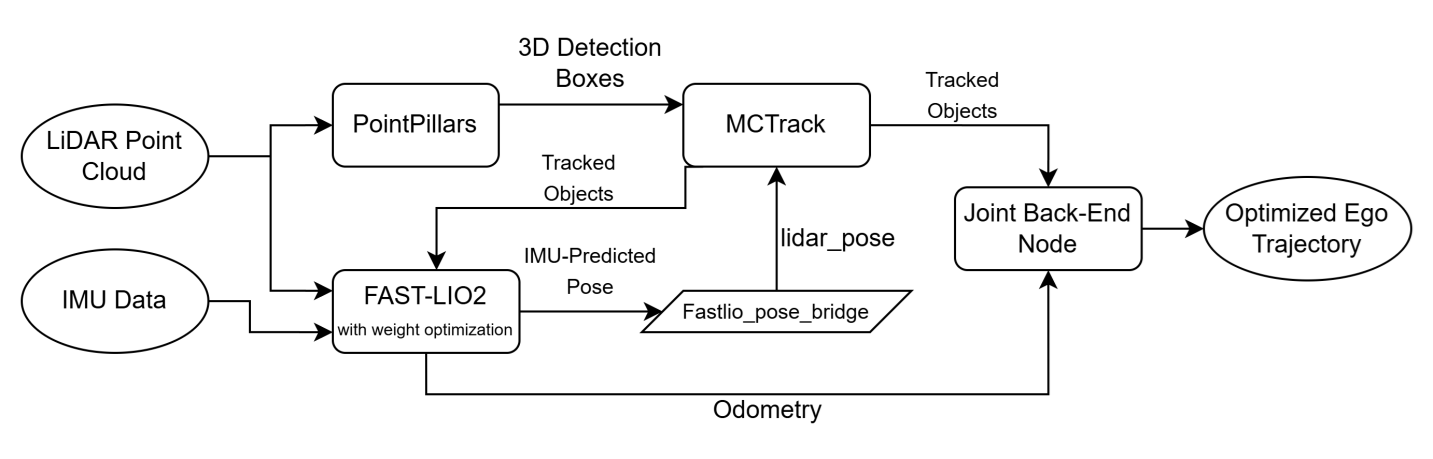
\includegraphics[width=0.96\textwidth]{Overall architecture of the proposed dynamic-scene trajectory optimization framework.png}
    \caption{系统总体架构图。展示了前端感知、中端双向融合与后端联合优化的完整协同管线。}
    \label{fig:overall_architecture}
\end{figure}

从整体结构看，项目实现的是一个三层协同系统：前端感知层、中端双向融合层和后端联合优化层。其输入来自 KITTI Tracking 转换得到的 rosbag，核心原始话题为 LiDAR 点云 \texttt{/kitti/velo/pointcloud} 与 IMU 数据 \texttt{/kitti/oxts/imu}。前端感知层同时运行 PointPillars 检测器与 FAST-LIO。PointPillars 的职责是从每帧点云中估计 3D 检测框，并输出统一消息类型 \texttt{Detection3DArray}；FAST-LIO 的职责是完成激光惯性里程计推算，并输出经滤波优化后的 \texttt{/Odometry} 以及更高频、早于 LiDAR 更新发布的 \texttt{/Odometry\_imu\_predicted}。

中端双向融合层是系统的关键枢纽。首先，通过 \texttt{fastlio\_pose\_bridge.py}，FAST-LIO 的里程计结果被转换为 MCTrack 可直接消费的 LiDAR 位姿 \texttt{/mctrack/lidar\_pose} 与 TF 变换。MCTrack 在线节点接收 \texttt{/detection/lidar\_detections} 和 \texttt{/mctrack/lidar\_pose}，在内部完成位姿插值、检测框坐标变换、目标关联和状态更新，然后向外发布 \texttt{/mctrack/tracked\_objects} 与可视化 Marker。其次，FAST-LIO 订阅 \texttt{/mctrack/tracked\_objects}，根据每个被跟踪目标的速度、加速度、置信度、尺寸和姿态信息，对落入动态框内的点云赋予更低权重。这样，目标跟踪结果不再只服务于感知显示，而是反向进入里程计优化。

后端联合优化层则进一步把这种双向交互从“前端数据权重调节”延伸到“后端位姿修正”。\texttt{joint\_backend\_ego\_node.py} 同时订阅 \texttt{/Odometry} 与 \texttt{/mctrack/tracked\_objects}，维护一个以自车位姿为变量的滑动窗口优化问题。在这个问题中，FAST-LIO 的相邻帧相对位姿提供里程计一致性约束，MCTrack 的目标观测提供对象一致性约束。优化结果只修正 ego 轨迹，不将目标作为显式优化变量，因此实现复杂度较低、计算代价受控，并通过 \texttt{/joint\_backend/odom} 发布最终轨迹。

从消息角度看，系统形成了非常明确的主链路：
\begin{itemize}
    \item LiDAR/IMU 原始数据进入 PointPillars 与 FAST-LIO；
    \item PointPillars 输出 \texttt{/detection/lidar\_detections}；
    \item FAST-LIO 输出 \texttt{/Odometry} 与 \texttt{/Odometry\_imu\_predicted}；
    \item Pose bridge 将 \texttt{/Odometry} 转为 \texttt{/mctrack/lidar\_pose}；
    \item MCTrack 结合检测与位姿输出 \texttt{/mctrack/tracked\_objects}；
    \item 跟踪结果一方面返回 FAST-LIO 做动态点降权，另一方面进入联合后端；
    \item 联合后端输出 \texttt{/joint\_backend/odom}，并交给评估脚本计算 ATE、RPE 和 KITTI 相对误差。
\end{itemize}

这条链路之所以成立，关键在于项目对消息结构进行了统一定义。检测消息 \texttt{Detection3D} 中包含帧号、类别、置信度、2D 包围框、3D 尺寸、位置和航向角；跟踪消息 \texttt{TrackedObject} 则进一步扩展了轨迹长度、全局姿态、LiDAR 坐标系姿态、融合速度、速度差分与加速度等字段。正是这些额外的运动信息，使后续的动态点降权和联合后端观测建模成为可能。

\section{前端感知层方法}
\subsection{PointPillars 三维目标检测}
本项目的检测前端采用 MMDetection3D 中的 PointPillars 实现，并在 \texttt{MMDET3D/local/ros/nodes/kitti\_pointpillars\_bag\_node.py} 中封装为可直接处理 rosbag 点云的 ROS 节点。该节点订阅 \texttt{/kitti/velo/pointcloud} 与 \texttt{/kitti/oxts/imu}，初始化 \texttt{LidarDet3DInferencer}，利用配置文件和权重完成 3D 检测推理。PointPillars 的核心思想是将稀疏点云编码为二维柱状表示，在保持较高速度的同时获得较好的检测精度，这非常适合课程项目中的在线运行需求。

与直接调用离线检测脚本不同，该 ROS 节点做了几件对全系统极为重要的工程工作。第一，它从 KITTI 标定文件中读取 \texttt{Tr\_velo\_cam} 与投影矩阵 \texttt{P2}，保证检测结果与坐标转换逻辑一致。第二，它将原始推理输出统一转换为系统内部定义的 \texttt{Detection3DArray} 消息，并同时发布 Marker、KITTI tracking 格式字符串和 LiDAR 坐标系格式字符串，便于不同模块兼容。第三，它保留了较低的检测置信度门限，默认 \texttt{confidence\_threshold} 为 0.05，这意味着检测节点尽量不过早裁剪候选框，把更多的筛选任务留给后续跟踪器完成。第四，它支持类别过滤和时序日志统计，使系统在调试不同类别组合、排查性能瓶颈时更容易定位问题。

从系统角度看，这样的设计有两个直接好处。其一，PointPillars 与 MCTrack 的接口不再依赖论文或第三方库中的原始格式，而是被标准化成带时间戳的 LiDAR 检测消息；其二，检测器与 FAST-LIO 使用同一份点云输入，因此时间对齐问题更容易追踪，不需要在多路异构感知流之间额外做复杂同步。

\subsection{FAST-LIO 激光惯性里程计}

\begin{figure}[H]
    \centering
    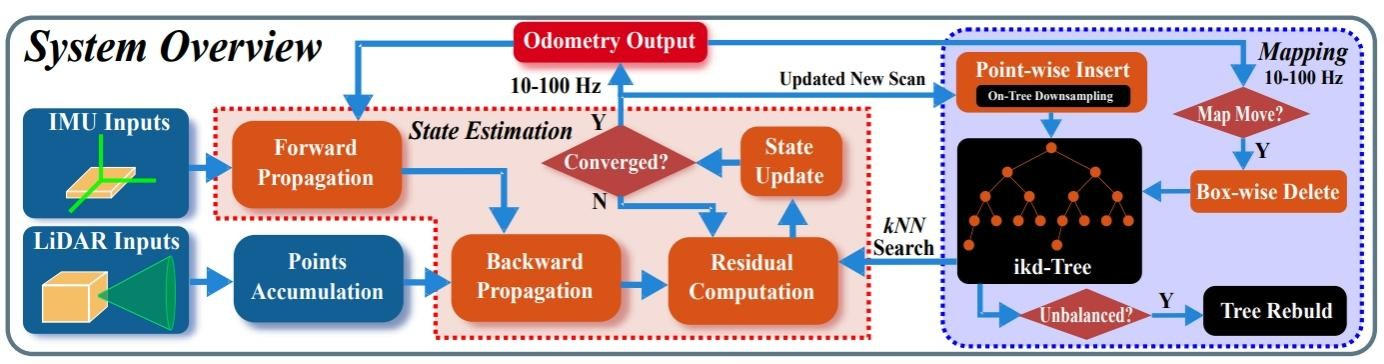
\includegraphics[width=0.8\textwidth]{FAST-LIO2 System Architecture.jpg}
    \caption{FAST-LIO2 系统架构图。本系统在其点到面残差计算环节引入了动态目标的自适应降权。}
    \label{fig:fastlio_architecture}
\end{figure}

定位前端采用 FAST-LIO，其核心是基于误差状态扩展卡尔曼滤波与点到面约束的 LiDAR-inertial 紧耦合里程计。与许多仅依赖点云配准的 SLAM 方法不同，FAST-LIO 在 IMU 高频积分与 LiDAR 更新之间建立了更紧密的状态传播关系，因此在高速运动、短时遮挡或几何退化场景下通常具有更强鲁棒性。本项目在 \texttt{catkin\_ws/src/fast\_lio/config/velodyne.yaml} 中配置其话题、外参、点云线数、扫描频率和建图参数；在 \texttt{mapping\_velodyne.launch} 中进一步控制是否启用动态权重机制。

仓库当前配置中，FAST-LIO 订阅 \texttt{/kitti/velo/pointcloud} 和 \texttt{/kitti/oxts/imu}，默认采用 64 线 Velodyne、10Hz 扫描率，LiDAR 外参平移为 \([0,0,0.28]\)，并发布优化位姿 \texttt{/Odometry} 以及 IMU 预测位姿 \texttt{/Odometry\_imu\_predicted}。其中 \texttt{/Odometry} 可以视为完成当前帧激光更新后的更可信位姿，而 \texttt{/Odometry\_imu\_predicted} 则更高频地反映 LiDAR 更新前的运动传播结果。后者对纯定位系统未必关键，但对目标跟踪非常有价值，因为目标跟踪本质上需要在两帧检测之间持续获得自车运动估计，才能在急转弯或高速情况下保持预测稳定。

本项目对 FAST-LIO 的修改重点并不在其主体滤波器，而在前处理与残差线性化阶段植入了动态权重机制。这意味着项目既保留了 FAST-LIO 原始前端的优点，又为动态目标反馈预留了自然接口。也正因为前端足够稳定，整个系统才能在此之上叠加跟踪和联合后端，而不至于因为底层里程计本身太脆弱而失去意义。

\subsection{Pose Bridge：从里程计到跟踪器位姿}
为了让 MCTrack 在 LiDAR 坐标系下正确解释检测框，本项目增加了 \texttt{fastlio\_pose\_bridge.py} 这一桥接节点。该节点订阅 FAST-LIO 发布的 \texttt{/Odometry}，读取 LiDAR 相对 IMU 的外参矩阵，将机体系位姿转换为 LiDAR 传感器原点位姿，并发布为 \texttt{/mctrack/lidar\_pose}。如果启用 \texttt{publish\_tf}，该节点还同步广播世界到 LiDAR 的 TF 变换。

这个节点虽然实现简单，但在整个系统中不可替代。原因在于，FAST-LIO 内部状态通常定义在 IMU 或机体系上，而 PointPillars 检测框直接输出于 LiDAR 坐标系。如果不经过这一步统一，MCTrack 就必须在内部自行推测或硬编码位姿坐标系，很容易导致全局变换与局部检测不一致。Bridge 节点把这个问题前置并显式化，使得跟踪器始终消费“与检测框严格同源坐标系”的位姿输入。

\section{中端双向融合方法}
\subsection{MCTrack 在线多目标跟踪}

\begin{figure}[H]
    \centering
    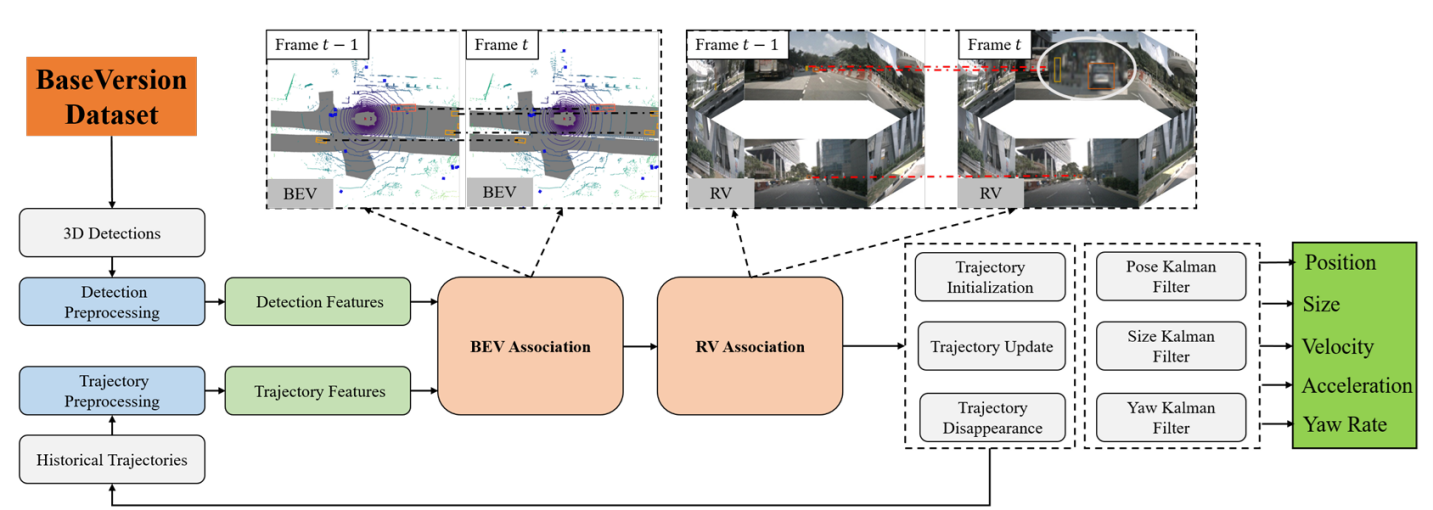
\includegraphics[width=0.8\textwidth]{Overview of 3D MOT framework MCTrack.png}
    \caption{MCTrack 多目标跟踪框架。在此基础上，本项目增加了带时间戳的位姿缓存与外推机制，以解决真实在线系统中的时滞问题。}
    \label{fig:mctrack_architecture}
\end{figure}

项目中的 MCTrack 在线节点位于 \texttt{catkin\_ws/src/ME5400/scripts/mctrack\_online\_node.py}。该节点加载 MCTrack 原始配置文件，维护一个 \texttt{Base3DTracker} 实例，并通过 \texttt{/mctrack/lidar\_pose} 接收自车位姿，通过 \texttt{/detection/lidar\_detections} 接收 PointPillars 检测结果。与简单的“检测来一帧就立刻送入跟踪器”不同，该实现专门构造了位姿缓存与待处理检测队列，以解决真实 ROS 管线中的时序错位问题。

具体而言，节点维护一个长度可配置的位姿缓冲区 \texttt{pose\_buffer}，每当收到新的 \texttt{PoseStamped}，就把时间戳与位姿矩阵存入缓存。检测回调收到 \texttt{Detection3DArray} 后不会盲目立即处理，而是先进入 \texttt{pending\_detections} 队列，然后尝试在缓存中寻找与检测时间戳最匹配的两帧位姿。如果检测时刻落在两帧位姿之间，则通过球面线性插值和位移线性插值得到中间位姿；如果短时间内仍匹配不到，则在超时后回退到最近位姿。这个设计直接提升了检测与位姿的时间一致性，是在线跟踪质量稳定的重要前提。

在坐标处理上，MCTrack 节点将 LiDAR 坐标系下的检测框通过 \texttt{lidar2global} 变换投影到全局坐标系，得到每个目标的 \texttt{global\_xyz}、\texttt{global\_yaw} 和全局朝向四元数，同时保留原始的 \texttt{lidar\_xyz} 与 \texttt{lidar\_yaw}。这样做的好处是，跟踪器可以在全局参考系中维护连续轨迹，而后续 FAST-LIO 动态降权又能够直接使用同一目标在 LiDAR 局部坐标系下的位置和姿态。跟踪输出消息 \texttt{TrackedObject} 中不仅包含 \texttt{track\_id} 与 \texttt{track\_length}，还包含 \texttt{velocity}、\texttt{velocity\_fusion}、\texttt{velocity\_diff}、\texttt{velocity\_curve} 与 \texttt{acceleration} 等多个运动字段，这些信息在后续模块中会被进一步利用。

从设计目标来看，MCTrack 在本项目中既承担传统 MOT 的目标连续性维护职责，又扮演连接检测与定位的中间层角色。一方面，FAST-LIO 提供的位姿帮助它完成运动补偿和更稳定的全局轨迹估计；另一方面，它输出的速度、置信度、尺寸与姿态信息又被 FAST-LIO 和联合后端再次使用。这一双向依赖关系，使 MCTrack 不再是单纯的“展示轨迹”的附属模块，而是成为整个闭环中的信息融合节点。

\subsection{FAST-LIO $\rightarrow$ MCTrack：高频位姿辅助跟踪}
在双向闭环的第一条链路上，FAST-LIO 对 MCTrack 的帮助主要体现在运动补偿。道路场景中，自车运动对检测框跨帧位置变化的影响往往不小于目标自身运动。如果忽略这一点，目标在图像或点云中的位置变化会被混合成“目标运动 + 自车运动”的叠加量，导致速度估计失真。FAST-LIO 提供的高频位姿，特别是 \texttt{/Odometry\_imu\_predicted} 这样的预测位姿，使跟踪器能够更及时地理解自车状态变化。

虽然当前在线节点主要通过桥接后的 \texttt{/mctrack/lidar\_pose} 消费校正后的里程计，但项目整体逻辑中已经明确保留了利用高频预测位姿进行运动补偿的能力。其价值在高速转弯场景中尤其明显：当相邻两帧点云间角速度较大时，如果跟踪器只知道较低频的 LiDAR 更新位姿，它对目标下一时刻位置的预测就会滞后；而引入更细粒度的位姿传播后，目标关联搜索区域可被显著缩小，轨迹更稳定、漏跟更少。

\subsection{MCTrack $\rightarrow$ FAST-LIO：动态目标自适应降权}
双向闭环的第二条链路是本项目当前最具代表性的创新点，即利用跟踪结果反向调节 FAST-LIO 对动态点的信任程度。其实现分布在 \texttt{laserMapping.cpp} 与 \texttt{preprocess.cpp} 中。FAST-LIO 订阅 \texttt{/mctrack/tracked\_objects} 后，会把每个目标转换为内部的 \texttt{DynamicObject} 结构，其中包括目标中心、包围盒半尺寸、局部航向角以及动态权重。这里的半尺寸并不等于原始目标尺寸的一半，而是在原始尺寸基础上额外加上 \(xy\) 与 \(z\) 方向的边界冗余，用于覆盖检测框与真实物体外轮廓之间的偏差。

动态权重的计算并不是拍脑袋设定，而是直接对应代码中的属性归一化与惩罚项设计。设目标速度为 \(v\)，加速度为 \(a\)，检测置信度为 \(s\)，则系统首先将它们分别归一化到 \([0,1]\) 范围，再根据参数 \(\alpha_v\)、\(\alpha_a\)、\(\alpha_s\) 形成惩罚项：
\begin{equation}
p = \alpha_v \cdot \mathrm{clamp}\left(\frac{v}{v_{\mathrm{ref}}}\right)
+ \alpha_a \cdot \mathrm{clamp}\left(\frac{a}{a_{\mathrm{ref}}}\right)
+ \alpha_s \cdot \mathrm{clamp}(s).
\end{equation}
随后得到目标权重
\begin{equation}
w = \mathrm{clip}(1-p,\; w_{\min},\; 1).
\end{equation}
当前仓库默认参数为 \(v_{\mathrm{ref}}=12.0\)、\(a_{\mathrm{ref}}=4.0\)、\(\alpha_v=0.5\)、\(\alpha_a=0.3\)、\(\alpha_s=0.2\)、\(w_{\min}=0.2\)。这意味着目标越快、加速度越大、检测置信度越高，就越可能被视作“真正动态且可信的动态目标”，从而被分配更小的权重。

权重注入发生在点云预处理阶段。对于每个输入点，系统检查它是否落入任一动态目标包围盒内部；如果是，则将该点的 \texttt{intensity} 更新为动态权重与原始 \texttt{intensity} 的较小值。这样做看似“借用了强度字段”，本质上却非常巧妙：因为 FAST-LIO 后续本就沿用点结构中的 \texttt{intensity} 字段，项目无需重新设计大规模数据结构，就能把动态权重一路带到映射与残差计算阶段。在线性化时，系统进一步将该权重作用于雅可比矩阵与点到面的残差项，相当于在滤波更新中弱化了来自动态点的影响。

这一机制相较于“硬剔除动态点”有两个实际优势。第一，它保留了过渡区域或边界点在某些时刻仍然可能提供的几何信息，不至于因为分割不完美而损失过多有效约束。第二，它允许根据目标运动属性连续调节，而不是二值地“要么保留，要么删除”。在工程系统中，这种软降权通常比硬阈值更鲁棒，也更容易调参。

\section{后端联合优化方法}
前端双向协同已经能显著改善建图质量，但本项目没有停留在“让前端更干净”这一层，而是进一步提出了一个 ego-only 滑窗联合后端，用于显式利用动态目标观测修正自车位姿。该模块实现于 \texttt{joint\_backend\_ego\_node.py}，对应配置文件为 \texttt{joint\_backend\_ego.yaml}。当前默认参数包括：窗口长度 8 帧、对象因子权重系数 \(\lambda_{\mathrm{obj}}=0.12\)、目标置信度阈值 0.6、最小轨迹长度 5、最大允许时间差 0.1\,s、最大速度突变 2.0\,m/s、对象权重下限 0.03，以及 Huber 鲁棒核尺度 0.5。

从优化变量看，这个后端只优化窗口内的自车平面位姿 \(\mathbf{p}_i=[x_i,y_i,\psi_i]^\top\)，并不把目标状态纳入变量集合。这一点与典型的紧耦合因子图工作不同，也正是其实现轻量、易于在线运行的重要原因。尽管如此，它仍然建立了两类关键残差。

第一类是里程计一致性残差。设窗口内第 \(i-1\) 帧和第 \(i\) 帧的自车位姿分别为 \(\mathbf{p}_{i-1}\) 和 \(\mathbf{p}_{i}\)，FAST-LIO 提供的相对运动观测记为 \(\hat{\mathbf{u}}_i\)，则该残差约束优化变量所对应的相对位姿应与 FAST-LIO 原始输出一致。系统进一步读取 \texttt{/Odometry} 中的协方差，当协方差异常或缺失时回退到预设噪声 \([0.20,0.20,0.10]\)，从而构造各维权重。

第二类是目标观测一致性残差。对于窗口中每一帧，后端在跟踪缓冲区中寻找时间戳最接近的目标快照，并仅保留满足轨迹长度、置信度、速度突变和时间同步门控的观测。对每个通过筛选的目标，系统先利用其速度把目标世界坐标外推到当前帧时刻，再将此外推后的世界位姿投影到当前优化中的自车局部坐标系下，得到预测观测 \(z^{\mathrm{pred}}_{ik}\)。实际观测 \(z^{\mathrm{meas}}_{ik}\) 则直接来自 \texttt{TrackedObject} 中记录的 LiDAR 局部位置与航向角。二者之差即构成对象残差：
\begin{equation}
r^{\mathrm{obj}}_{ik}=z^{\mathrm{pred}}_{ik}-z^{\mathrm{meas}}_{ik}.
\end{equation}

综合起来，窗口优化目标可写为
\begin{equation}
\min_{\{\mathbf{p}_i\}}
\sum_{i=2}^{N}\|r^{\mathrm{odom}}_i\|_{W_i}^2
\;+\sum_{i=1}^{N}\sum_{k\in\mathcal{V}_i}
w_{ik}\,\rho\!\left(\|r^{\mathrm{obj}}_{ik}\|_2^2\right),
\end{equation}
其中 \(\mathcal{V}_i\) 表示第 \(i\) 帧通过门控的目标集合，\(\rho(\cdot)\) 为 Huber 或 Cauchy 鲁棒核。对象因子的权重 \(w_{ik}\) 由检测得分、轨迹长度归一化值以及全局系数 \(\lambda_{\mathrm{obj}}\) 共同决定，代码中采用了一个具有下限约束的平方根型组合方式，以避免对象因子整体过弱而失去作用。

与很多“大而全”的联合图优化不同，这个后端的思想非常务实。它并不试图重建完整的目标状态图，也不追求从数学上一次性解决 SLAM 与 MOT 的全部耦合问题，而是利用稳定跟踪车辆充当“临时移动锚点”。如果自车位姿偏了，那么在当前位姿估计下看到的目标相对位置就会偏；反过来，最小化这种偏差就能拉回自车轨迹。由于目标状态来自现有跟踪器，这种做法以很低的开发成本验证了“动态目标信息可以帮助自车定位”这一关键命题。

当然，这种 ego-only 方案也有天然局限。目标世界位置不是优化变量，而是由跟踪器给出的点估计并经速度传播得到，因此若目标状态本身不可靠，优化会把错误目标当成参考物。序列 0011 的退化结果正说明了这一点：当基线已足够好、可用动态目标又不够强时，引入对象约束可能带来过修正。换句话说，这个后端已经证明“利用目标帮助定位”有价值，但也清楚暴露出后续需要更强门控与更自适应激活策略。

\section{工程实现与运行流程}
除了算法模块，本项目的一大特点是工程链路完整。仓库通过 \texttt{Scripts/} 目录对不同子系统的启动脚本进行了分类管理，包括 PointPillars、FAST-LIO、MCTrack、联合后端、离线 feeder、RViz 和评估脚本等。最上层脚本 \texttt{run\_all.sh} 会顺序执行两套流程：先运行纯净基线 \texttt{run\_baseline.sh}，再运行带感知闭环的优化流程 \texttt{run\_optimized.sh}，并把所有日志统一写入 \texttt{Results/<seq>\_results/full\_run.log}。这种双轨连跑设计非常适合课程项目，因为它天然控制了变量，使基线与优化版在同一套数据、同一套启动逻辑下可直接对比。

为了应对“检测器算不过来导致 rosbag 已经播完、下游节点却还没处理完”的典型离线问题，项目还实现了 \texttt{offline\_bag\_feeder.py}。它不是简单地替代 \texttt{rosbag play}，而是采用一种半同步调度方式：每发布一帧 LiDAR 点云，就等待同一时间戳附近的检测结果和跟踪结果完成，期间以固定步长推进 \texttt{/clock}，从而让整个系统在仿真时间下保持同步。脚本中为检测和跟踪分别设置超时门限、时间戳容忍度与轮询频率，因此即便下游偶尔波动，也不会让全流程永久卡死。这一设计在使用深度学习检测器进行离线评估时非常关键，因为它显著降低了丢帧和错时带来的实验噪声。

评估方面，项目提供了两类脚本。一类是 \texttt{evaluate\_joint\_backend.py}，使用时间戳匹配与 Umeyama 对齐计算 ATE 和平移型 RPE，并绘制论文风格的轨迹与误差图。另一类是 \texttt{evaluate\_kitti\_tr\_rot.py}，依据 KITTI 传统里程计协议计算不同路径长度下的相对平移误差和旋转误差。这使项目既能从“全局轨迹贴近真值的程度”评价系统，也能从“单位路径长度上的局部误差”观察改动是否改善了短时稳定性。对课程项目而言，这种双指标体系比只看单一 RMSE 更有解释力，因为动态点降权和联合后端不一定同时改善所有指标。

在可视化方面，仓库提供了统一的 RViz 配置文件 \texttt{Scripts/rviz/ME5400.rviz}，用于同时显示原始点云、PointPillars 检测框、MCTrack 跟踪框、FAST-LIO 地图与联合后端轨迹。再加上 \texttt{cleanup\_ros\_runtime.sh} 这样的运行时清理脚本，整个项目已经具备较完善的开发闭环：可以一键运行、分模块调试、离线重放、可视化检查、量化评估和结果归档。

\section{实验设计与结果分析}
\subsection{实验设置}
本报告实验部分统一采用仓库 \texttt{Results/} 中当前可核对的结果。主对比任务为两轨实验：\texttt{Baseline(Offline,NoWeight)} 与 \texttt{JointOffline}。其中，前者表示关闭动态权重与联合后端的纯 FAST-LIO 基线；后者表示启用 PointPillars、MCTrack、动态点降权和 ego-only 联合后端的完整系统。需要强调的是，这里的 \texttt{JointOffline} 并不是“只多了一个后端优化器”，而是对应整个协同链路全部打开后的结果，因此它体现的是“检测 + 跟踪 + 前端反馈 + 后端修正”的综合收益。

实验数据来自 KITTI Tracking 多个序列。仓库当前给出了 0001、0007、0009、0011、0020 五个序列的联合后端指标和 KITTI 相对误差指标，足以观察系统在不同场景中的稳定性差异。根据 README 对数据的说明，0020 是高速场景，0019、0009 等则更偏城市街道。不同工况下，动态目标密度、可用静态结构比例以及自车运动模式都不同，这会直接影响本项目这种“同时依赖静态结构与动态目标信息”的系统表现。

\begin{figure}[H]
    \centering
    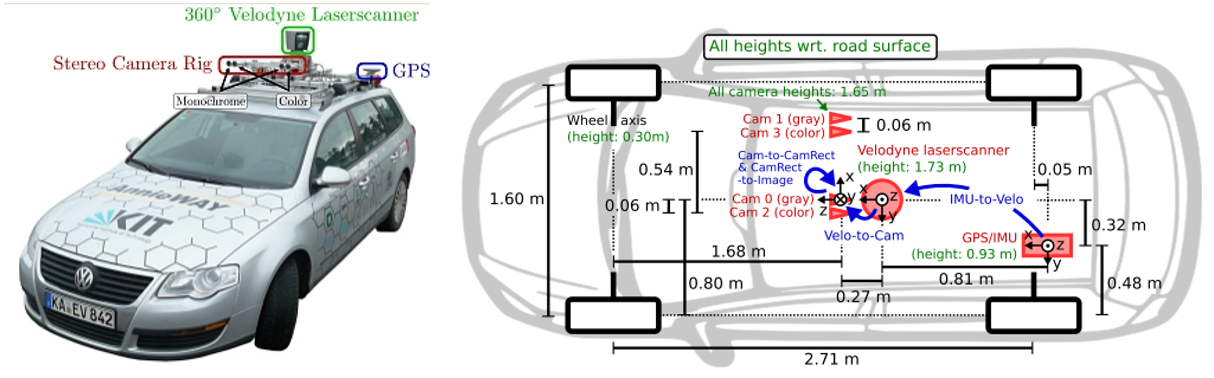
\includegraphics[width=0.6\textwidth]{The KITTI data collection vehicle.png}
    \caption{KITTI 数据采集平台。}
    \label{fig:kitti_vehicle}
\end{figure}

\subsection{主结果：序列 0020}
图~\ref{fig:joint_eval} 展示了仓库中 \texttt{evaluation\_joint\_backend.png} 的结果，可看出完整系统在 0020 序列上显著贴近真值轨迹。根据 \texttt{metrics\_joint\_backend.txt}，基线 ATE RMSE 为 29.1782\,m，联合系统降至 11.5856\,m，改善 60.29\%；ATE 均值从 26.3322\,m 降至 10.0928\,m，ATE 最大值从 39.9080\,m 降至 17.4796\,m。根据 \texttt{metrics\_kitti\_tr\_rot\_ac.txt}，KITTI 相对平移误差由 6.0245\% 降至 2.9930\%，改善 50.32\%；旋转误差由 0.6357\,deg/100m 降至 0.5312\,deg/100m，改善 16.44\%。

\begin{figure}[H]
    \centering
    
\includegraphics[width=0.96\textwidth]{evaluation_joint_backend.png}
    \caption{序列 0020 的联合后端评估图。上图为 Umeyama 对齐后的轨迹对比，中图为 ATE 随帧变化，下图为单帧平移型 RPE。可以看到完整系统显著降低了全局漂移，但对局部 RPE 的改善不如 ATE 那样统一。}
    \label{fig:joint_eval}
\end{figure}

这个结果非常符合系统设计预期。首先，0020 是一个动态影响较重且累计漂移显著的序列，因此动态点降权能够有效压制错误地图更新，减少“把运动目标写进静态地图”带来的长期偏差。其次，联合后端通过目标观测一致性约束进一步抑制了长时漂移，使优化轨迹更贴近真值。再者，从 RPE 曲线看，完整系统并没有把所有局部误差都消灭，说明当前系统的主要优势在于“压制累计偏移”，而非完全重塑每一帧的局部配准质量。

\subsection{多序列结果}
表~\ref{tab:ate_multi} 总结了仓库当前五个序列的 ATE 指标。可以看到，系统在 0001、0007、0009、0020 上均优于基线，且在 0020 上收益最大；但在 0011 上出现了明显退化。表~\ref{tab:kitti_multi} 则给出 KITTI 相对误差结果。与 ATE 不同，平移与旋转相对误差并非在所有序列上都改善，说明系统当前更偏向通过动态信息降低全局偏移，而不是统一改善所有局部段误差。

\begin{table}[H]
    \centering
    \caption{多序列 ATE 结果汇总}
    \label{tab:ate_multi}
    \begin{tabular}{ccccccc}
        \toprule
        序列 & 基线 RMSE & 联合 RMSE & 改善 & 基线均值 & 联合均值 & 备注 \\
        \midrule
        0001 & 2.3343 & 1.7317 & +25.82\% & 2.1035 & 1.5658 & 改善明显 \\
        0007 & 3.3231 & 2.6958 & +18.88\% & 3.2743 & 2.4254 & 中等改善 \\
        0009 & 2.4151 & 2.0039 & +17.03\% & 2.3277 & 1.9321 & 小幅改善 \\
        0011 & 0.4965 & 1.0479 & -111.07\% & 0.4125 & 0.8060 & 失败案例 \\
        0020 & 29.1782 & 11.5856 & +60.29\% & 26.3322 & 10.0928 & 最显著 \\
        \bottomrule
    \end{tabular}
\end{table}

\begin{table}[H]
    \centering
    \caption{多序列 KITTI 相对误差结果汇总}
    \label{tab:kitti_multi}
    \begin{tabular}{cccccc}
        \toprule
        序列 & 基线 Tr.(\%) & 联合 Tr.(\%) & 改善 & 基线 Rot. & 联合 Rot. \\
        \midrule
        0001 & 4.4355 & 3.3913 & +23.54\% & 2.0336 & 1.5419 \\
        0007 & 2.5718 & 2.8668 & -11.47\% & 1.8037 & 2.3480 \\
        0009 & 2.6519 & 3.1584 & -19.10\% & 1.3420 & 1.5859 \\
        0011 & 1.2282 & 1.5713 & -27.93\% & 0.6825 & 0.7314 \\
        0020 & 6.0245 & 2.9930 & +50.32\% & 0.6357 & 0.5312 \\
        \bottomrule
    \end{tabular}
\end{table}

这些结果揭示出项目当前方法的几个特点。第一，系统对“长期轨迹偏移较大、动态目标较多”的序列更有效。例如 0020 上改善幅度远高于其他序列，这说明当前方法的主要收益来自动态点污染抑制与目标辅助的全局漂移校正。第二，当基线已经足够准确时，额外引入目标约束未必总是有利。0011 的基线 ATE RMSE 只有 0.4965\,m，说明原始 FAST-LIO 已经表现很好，此时对象约束一旦含噪，收益就可能被副作用抵消。第三，相对误差指标在部分序列上退化，说明系统并不一定在短窗口尺度上更平滑。换句话说，当前联合后端更像一个“长时漂移纠偏器”，而不是一个通用的局部精修器。

\subsection{失败案例与原因分析}
序列 0011 的退化是当前系统最值得认真分析的案例。首先，该序列本身基线误差很低，意味着场景中的静态几何已经足够支持 FAST-LIO 获得稳定定位。此时，如果系统强行加入目标约束，优化问题就可能从“引入补充信息”变成“引入多余且可能带噪的信息”。其次，当前后端只优化 ego 位姿，目标世界状态并未一并优化，而是依赖跟踪器给出的速度传播预测。如果目标存在短时非匀速运动、局部遮挡、检测框抖动或者速度估计偏差，这些误差会直接传递到对象残差中。再次，当前对象门控虽然已经包含置信度、轨迹长度、速度突变和时间差限制，但仍然是静态规则，尚未做到根据场景难度、基线稳定度和目标数量动态调节。

从工程角度看，这个失败案例并不是坏消息。相反，它说明系统已经进入“不是任何时候都该激活所有约束”的更细阶段。真正成熟的系统应当学会在不同场景下自适应启停或重加权对象因子。例如，当基线协方差持续较小且场景静态结构丰富时，可以降低或关闭对象约束；当 FAST-LIO 检测到几何退化、漂移增长或动态目标轨迹非常稳定时，再逐步提高对象约束权重。这样的策略能够让系统更像一个条件激活的协同优化器，而不是固定参数下的全程附加模块。

\section{局限性与未来工作}
尽管本项目已经完成了一个从检测、定位、跟踪到联合优化的闭环系统，但它仍然存在若干明确局限。第一，系统总体上仍属于松耦合架构。各模块通过 ROS topic 通信，虽然维护方便，但信息利用深度有限。例如，FAST-LIO 内部并不直接感知目标轨迹协方差，MCTrack 也无法反向读取里程计状态不确定性。第二，联合后端只优化 ego 位姿，不优化目标状态，因此无法在统一图中同时消解自车与目标的不确定性。第三，当前动态点处理仍然停留在“权重调节”的层面，尚未真正把动态物体表面的刚体结构提炼为可重复利用的几何约束。第四，实验规模仍然有限，目前只有若干 KITTI 序列的结果，还不足以对不同类型场景做全面统计结论。

未来工作可以从三个方向推进。第一个方向是把当前 ego-only 后端扩展为更完整的滑窗联合图优化，将自车位姿、目标位姿甚至 IMU 偏置共同纳入变量集合，并引入更系统的边缘化机制。第二个方向是继续深化“动态物体即移动路标”的思路，不只使用目标框中心和速度，而是尝试利用动态车辆表面点云的刚体一致性构造 object-centric 因子。若这一点能够真正落地，将使系统从“根据目标状态间接帮助定位”进一步走向“直接利用动态物体几何结构帮助定位”。第三个方向是建立自适应协同策略，根据 FAST-LIO 协方差、场景几何退化程度、目标数量与轨迹稳定度，自动决定何时启用对象约束、何时降低动态点权重、何时完全关闭附加优化。这些改进将决定项目能否从一个成功的课程工程系统，进一步成长为具有研究贡献的动态场景 LiDAR-inertial 联合优化框架。

\section{结论}
本报告围绕 ME5400 课程项目，系统总结了一套由 PointPillars、FAST-LIO、MCTrack 和 ego-only 联合后端组成的动态场景双向协同系统。项目的核心贡献不在于重新发明某个单独模块，而在于完成了多模块之间的信息闭环：FAST-LIO 的高质量位姿帮助 MCTrack 做运动补偿，MCTrack 的目标状态又反过来帮助 FAST-LIO 抑制动态点污染，并通过联合后端进一步修正自车轨迹。实验结果表明，该系统在多个 KITTI Tracking 序列上具有实际收益，尤其在序列 0020 上显著降低了全局轨迹误差和相对平移误差。

更重要的是，项目已经清楚展示出一个研究上很有价值的方向：动态物体不应只被当成需要过滤的噪声，它们在满足足够稳定性和可观测性的前提下，可以转化为帮助定位的对象级约束。当前实现还只是这一方向的工程起点，但它已经证明了完整链路的可行性，也为后续更强的 LiDAR-inertial object-centric 联合优化提供了扎实基础。

\begin{thebibliography}{9}
\bibitem{fastlio2}
W. Xu, Y. Cai, D. He, J. Lin, and F. Zhang, ``FAST-LIO2: Fast direct LiDAR-inertial odometry,'' \emph{IEEE Transactions on Robotics}, vol. 38, no. 4, pp. 2053--2073, 2022.

\bibitem{pointpillars}
A. H. Lang, S. Vora, H. Caesar, L. Zhou, J. Yang, and O. Beijbom, ``PointPillars: Fast encoders for object detection from point clouds,'' in \emph{Proc. CVPR}, 2019, pp. 12697--12705.

\bibitem{kitti}
A. Geiger, P. Lenz, and R. Urtasun, ``Are we ready for autonomous driving? The KITTI vision benchmark suite,'' in \emph{Proc. CVPR}, 2012, pp. 3354--3361.

\bibitem{ab3dmot}
X. Weng, J. Wang, D. Held, and K. Kitani, ``3D multi-object tracking: A baseline and new evaluation metrics,'' in \emph{Proc. IROS}, 2020, pp. 10359--10366.
\end{thebibliography}

\end{document}
